\documentclass[conference]{IEEEtran}
\IEEEoverridecommandlockouts

\usepackage{cite}
\usepackage{amsmath,amssymb,amsfonts}
\usepackage{algorithmic}
\usepackage{graphicx}
\usepackage{textcomp}
\usepackage{xcolor}
\usepackage{booktabs}
\usepackage{multirow}
\usepackage{microtype}
\usepackage{url}
\usepackage{balance}

\def\BibTeX{{\rm B\kern-.05em{\sc i\kern-.025em b}\kern-.08em
    T\kern-.1667em\lower.7ex\hbox{E}\kern-.125emX}}

\begin{document}

\title{Attention-Augmented Residual Deep Learning Framework for Lymphoma Detection}

\author{
\IEEEauthorblockN{Bhuvanesh A U\IEEEauthorrefmark{1}, Likith Arya D\IEEEauthorrefmark{1}, Monisha K P\IEEEauthorrefmark{1}, Manthan Nayak\IEEEauthorrefmark{1}, and Sindhu K S\IEEEauthorrefmark{2}}
\IEEEauthorblockA{\IEEEauthorrefmark{1}Department of Information Science and Engineering, Malnad College of Engineering, Hassan, Karnataka, India\\
Email: \{bhuvaneshau2309, likhitharyad17, monishakp28, manthannayak1234567\}@gmail.com}
\IEEEauthorblockA{\IEEEauthorrefmark{2}Assistant Professor, Department of Information Science and Engineering, Malnad College of Engineering, Hassan, Karnataka, India\\
Email: sindhuks@mcehassan.ac.in}
}

\maketitle

\begin{abstract}
Microscopic examination of tissue biopsies remains a cornerstone in diagnosing mature B-cell lymphoid malignancies, including Chronic Lymphocytic Leukemia (CLL), Follicular Lymphoma (FL), and Mantle Cell Lymphoma (MCL). Differentiating these subtypes on Hematoxylin and Eosin (H\&E) stained histological sections is challenging because of overlapping nuclear features, high cellular density, and staining variations across laboratories. In this work, we investigate an attention-augmented residual learning framework for automated three-class lymphoma subtyping and input quality screening. The network integrates Convolutional Block Attention Modules (CBAM) after Stages~3 and~4 of a ResNet-50 backbone, allowing the model to adaptively weight informative feature channels and spatial nuclear regions. To retain both broader tissue context and localized nuclear peaks, feature maps are pooled using parallel Global Average Pooling (GAP) and Global Max Pooling (GMP) into a 4,096-dimensional vector before classification. An input screening module evaluates stain chromaticity in HSV space and edge density, combined with a decision confidence threshold ($\tau = 0.80$, selected via an empirical threshold sweep on an $N = 56$ validation partition) to flag non-histological or borderline inputs for manual review. Model interpretability is examined using Grad-CAM++ attribution maps. On a primary benchmark of 15,000 microscopic images partitioned at the image level into a 70:15:15 split ($N_{\text{test}} = 2,250$), the model achieved 100.00\% test accuracy and a macro ROC-AUC of 1.0000. When tested zero-shot on an independent external cohort of 374 microscopic biopsy images without fine-tuning, the network yielded a macro ROC-AUC of 0.8126 and a raw accuracy of 34.22\%, illustrating cross-domain stain shifts toward darker hematoxylin absorption. Controlled in-domain ablation on the clinical cohort ($N = 57$ test split) shows that spatial attention provides the primary accuracy gain (+7.01\% over baseline ResNet-50), with combined CBAM matching SAM in top-1 accuracy (85.96\%) while yielding a slight refinement in macro F1 (0.8568) and a macro ROC-AUC of 0.9401.
\end{abstract}

\begin{IEEEkeywords}
Digital Pathology, Lymphoma Subtype Classification, Convolutional Block Attention Module, Deep Residual Networks, Grad-CAM++, Computer-Aided Screening.
\end{IEEEkeywords}

\section{Introduction}
\IEEEPARstart{M}{alignant} lymphomas encompass a diverse spectrum of clonal lymphoproliferative disorders originating in the immune system~\cite{almekhlafi2023comprehensive, syrykh2020automated}. Among non-Hodgkin mature B-cell neoplasms, Chronic Lymphocytic Leukemia / Small Lymphocytic Lymphoma (CLL), Follicular Lymphoma (FL), and Mantle Cell Lymphoma (MCL) represent three frequently encountered subtypes that require distinct clinical management~\cite{guo2021research, alsadi2023enhanced}. Clinical pathways vary markedly across these conditions: CLL often permits watchful waiting or targeted kinase inhibition, FL typically responds to immunochemotherapy, and MCL commonly presents aggressively, requiring intensive multi-agent regimens~\cite{sharma2025enhancing, singh2023enhanced}.

In diagnostic pathology, tissue biopsies stained with Hematoxylin and Eosin (H\&E) are routinely evaluated under light microscopy~\cite{raman2025deep}. Pathologists assess cellular and architectural attributes, such as nuclear size, chromatin texture, membrane irregularity, nucleoli presence, and nodular versus diffuse growth patterns~\cite{sertel2010computer, kong2010detection}. However, manual visual grading is labor-intensive and prone to inter-observer variability, particularly in borderline cases where cytological boundaries between mature lymphoid cells appear subtle~\cite{sertel2013detection, taskiran2010automatic}. Computer-aided diagnostic systems offer practical utility by providing reproducible second opinions to assist clinical workflows~\cite{syrykh2020automated, sharma2025enhancing}.

Initial automated approaches focused on handcrafted texture descriptors, Fourier transforms, and morphological segmentation~\cite{taskiran2010automatic, sertel2012multi}. Although informative, these methods often struggle with variations in slice thickness, illumination, and staining protocols across laboratories~\cite{almekhlafi2023comprehensive}. Deep learning models, particularly convolutional networks such as ResNet~\cite{he2016deep}, DenseNet~\cite{huang2017densely}, and EfficientNet~\cite{tan2019efficientnet}, have addressed many of these limitations by learning hierarchical visual features directly from image data~\cite{guo2021research}.

\begin{figure*}[!t]
\centering
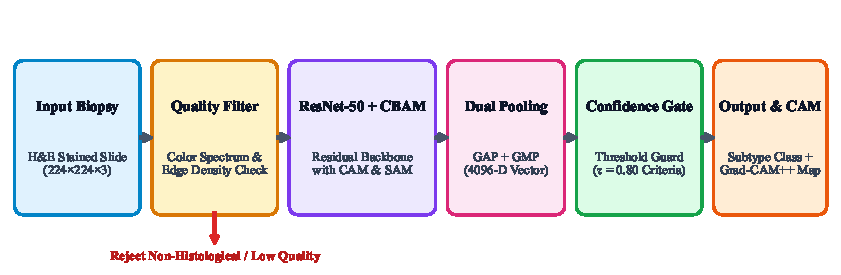
\includegraphics[width=0.90\textwidth]{figures/fig1_framework.pdf}
\caption{Workflow of the proposed lymphoma subtype classification and screening framework. Uploaded biopsy images undergo color chromaticity and edge density quality checks before feature extraction by a ResNet-50 backbone augmented with CBAM modules. Dual pooled features (GAP + GMP, 4,096-D) feed a regularized classification head with confidence-gated rejection ($\tau = 0.80$) and Grad-CAM++ visualization.}
\label{fig:framework}
\end{figure*}

Nevertheless, applying standard convolutional networks to microscopic biopsy subtyping involves practical challenges:
\begin{enumerate}
    \item \textit{Spatial and Channel Unselectivity:} Standard convolution kernels treat all spatial coordinates uniformly. In biopsy sections, non-diagnostic background glass, interstitial fluid, and red blood cells can distract the network from diagnostic lymphoid nuclei~\cite{raman2025deep}.
    \item \textit{Forced Softmax Outputs:} Standard classifiers normalize unconstrained output logits into class probabilities that sum to 1.0. Consequently, blurred images, non-histological inputs, or corrupted slides may still be assigned to a cancer class with high nominal confidence~\cite{singh2023enhanced}.
    \item \textit{Decision Opacity:} Deep representations lack direct visual explanation, making it difficult for pathologists to verify whether predictions rely on genuine cellular morphology or background slide artifacts~\cite{alsadi2023enhanced, chattopadhay2018grad}.
\end{enumerate}

To address these challenges, this paper presents an attention-augmented residual deep learning framework for lymphoma subtype classification (CLL, FL, MCL) with built-in screening safeguards. The main contributions of this work are:
\begin{itemize}
    \item We incorporate Convolutional Block Attention Modules (CBAM) after Stages~3 and~4 of ResNet-50, sequentially refining channel representations and highlighting spatial regions corresponding to lymphoid nuclei.
    \item We implement a dual pooling head that combines Global Average Pooling (GAP) and Global Max Pooling (GMP) into a 4,096-dimensional representation, preserving both overall tissue context and localized nuclear peak activations.
    \item We integrate an automated image quality assessment and confidence-gated screening guard ($\tau = 0.80$, selected on a validation partition) to flag corrupted inputs or borderline predictions for secondary review.
    \item We evaluate the framework on a primary benchmark of 15,000 microscopic images, examine generalization on an independent 374-image clinical cohort under cross-laboratory stain shifts, perform controlled ablation studies, and analyze visual heatmaps using Grad-CAM++.
\end{itemize}

The rest of the paper is organized as follows: Section~\ref{sec:related} discusses related work; Section~\ref{sec:methodology} describes the architecture, attention mechanisms, and screening pipeline; Section~\ref{sec:experiments} details the experimental setup; Section~\ref{sec:results} presents benchmark results, cross-domain evaluation, ablation studies, and Grad-CAM++ visualizations; Section~\ref{sec:limitations} discusses limitations; and Section~\ref{sec:conclusion} concludes the paper.

\section{Related Work}
\label{sec:related}

\subsection{Morphological Image Analysis in Histopathology}
Early efforts in computerized lymphoma diagnosis used handcrafted features extracted from digitized microscopy images. Taskiran and Kahya~\cite{taskiran2010automatic} applied steerable wavelets and discrete cosine transforms to classify non-Hodgkin lymphoma subtypes. Sertel et al.~\cite{sertel2010computer, sertel2012multi, sertel2013detection} introduced color-texture segmentation and Expectation-Maximization clustering to quantify centroblasts for grading follicular lymphoma. Kong et al.~\cite{kong2010detection} applied iterative watershed transforms on immunohistochemically stained sections to delineate follicular boundaries. While these methods offered interpretability, their sensitivity to illumination, tissue preparation, and stain color limits their consistency across laboratories.

\subsection{Deep Learning for Lymphoma Classification}
Convolutional neural networks have significantly improved histopathological classification. Guo et al.~\cite{guo2021research} used deep residual networks to classify lymphoma subtypes, finding that residual connections helped mitigate vanishing gradients. Al-Sadi et al.~\cite{alsadi2023enhanced} developed an explainable framework combining dilated MobileNetV2 with recurrent neural networks to capture sequential spatial dependencies. Sharma and Verma~\cite{sharma2025enhancing} applied transfer learning across multiple architectures, demonstrating the benefit of pre-trained feature extractors. Syrykh et al.~\cite{syrykh2020automated} evaluated whole-slide scanning workflows and highlighted the importance of representative training data across preparation centers. Comprehensive surveys by Al-Mekhlafi et al.~\cite{almekhlafi2023comprehensive} and Singh and Agrawal~\cite{singh2023enhanced} emphasize the need for architectures that balance high classification accuracy with interpretability and out-of-distribution detection.

\subsection{Attention Mechanisms and Visual Saliency}
Attention modules allow deep networks to prioritize informative feature subspaces. Woo et al.~\cite{woo2018cbam} introduced the Convolutional Block Attention Module (CBAM), combining channel and spatial attention with negligible computational overhead. Raman et al.~\cite{raman2025deep} applied self-attention mechanisms to hematological smear classification, demonstrating improved resilience to background staining variations.

For visual explanation, Selvaraju et al.~\cite{selvaraju2017grad} developed Grad-CAM, using gradient information to generate coarse localization maps. Chattopadhay et al.~\cite{chattopadhay2018grad} proposed Grad-CAM++, using a weighted average of positive partial derivatives to better localize multiple object instances and fine structural details. In this study, we use Grad-CAM++ to examine how attention-guided features correlate with diagnostic nuclear morphology.

\begin{figure*}[!t]
\centering
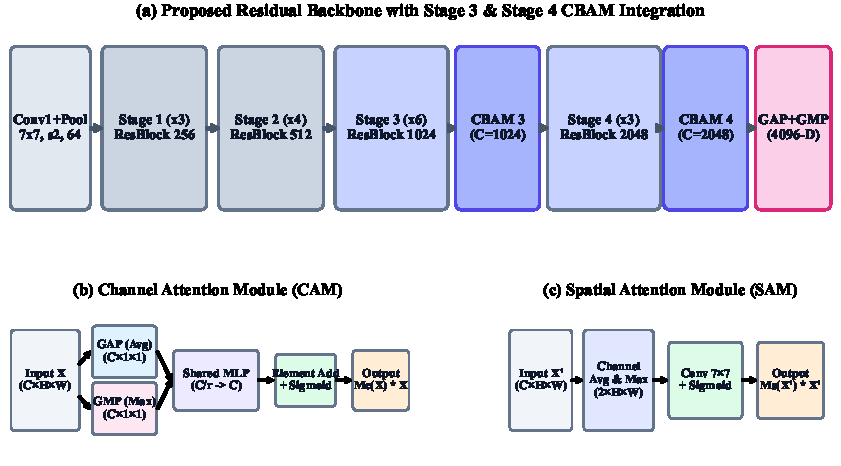
\includegraphics[width=0.90\textwidth]{figures/fig2_architecture.pdf}
\caption{Detailed architectural pipeline of the Attention-Augmented ResNet-50. Input images ($224 \times 224 \times 3$) pass through an initial $7 \times 7$ convolution (stride 2), max-pooling, and four residual stages. CBAM blocks are positioned after Stage~3 ($C=1024$) and Stage~4 ($C=2048$). Dual pooling (GAP + GMP) concatenates features into a 4,096-dimensional vector feeding a regularized classification head.}
\label{fig:architecture}
\end{figure*}

\section{Methodology}
\label{sec:methodology}

The end-to-end framework comprises four main components: an input quality screening module, a CBAM-augmented ResNet-50 backbone, a dual pooling classification head, and a confidence-gated decision mechanism with Grad-CAM++ visualization (Fig.~\ref{fig:framework}).

\subsection{Input Quality Assessment and Filtering}
To prevent non-diagnostic images from entering the network, inputs undergo heuristic quality checks based on tissue color chromaticity and edge density:
\begin{enumerate}
    \item \textit{Blank and Contrast Check:} Digital images are evaluated for extreme intensity and contrast deficiency. Images with mean intensity $\mu_I < 5.0$ (pitch black), $\mu_I > 250.0$ (blank white), or pixel standard deviation $\sigma_I < 8.0$ (uniform field) are rejected.
    \item \textit{Stain Chromaticity Check:} Histological sections stained with H\&E exhibit characteristic pink, magenta, purple, and blue hues, while natural foliage and environmental scenes contain green-yellow tones. In HSV color space (with Hue $H \in [0, 180]$), we define the non-histological foliage mask as $(26 \le H \le 88) \land (S \ge 25) \land (V \ge 25)$. If the fraction of pixels matching this mask exceeds 0.10, the input is rejected. Furthermore, the valid H\&E tissue and glass spectrum is defined as:
    \begin{equation}
    \label{eq:stain_mask}
    \mathcal{M}_{\text{stain}}(i,j) = (H \ge 95) \lor (H \le 25) \lor (S < 22)
    \end{equation}
    The stain concordance ratio is:
    \begin{equation}
    \label{eq:stain_ratio}
    R_{\text{stain}} = \frac{1}{H \times W} \sum_{i=1}^H \sum_{j=1}^W \mathbb{I}\big(\mathcal{M}_{\text{stain}}(i,j)\big)
    \end{equation}
    Inputs with $R_{\text{stain}} < 0.70$ are flagged as non-histological.
    \item \textit{Edge Density Check:} Microscopic biopsies contain dense nuclear boundaries producing high spatial-frequency gradients. Using Sobel horizontal ($g_x$) and vertical ($g_y$) operators on grayscale images, gradient magnitude is computed as $M(i,j) = \sqrt{g_x(i,j)^2 + g_y(i,j)^2}$. Edge density is:
    \begin{equation}
    \label{eq:edge_density}
    R_{\text{edge}} = \frac{1}{H \times W} \sum_{i=1}^H \sum_{j=1}^W \mathbb{I}\big(M(i,j) > 35\big)
    \end{equation}
    Inputs with $R_{\text{edge}} < 0.35$ are flagged as blurred or lacking cellular structure.
\end{enumerate}
These criteria serve as an operational heuristic pre-filter and have not been validated on a formal non-histological benchmark cohort.

\subsection{Attention-Augmented ResNet-50 Backbone}
The feature extraction backbone is built upon ResNet-50~\cite{he2016deep}, comprising an initial $7 \times 7$ convolution (stride 2), max-pooling, and four residual stages with 3, 4, 6, and 3 bottleneck blocks, respectively (Fig.~\ref{fig:architecture}).

To guide the network toward salient cellular morphology, CBAM modules~\cite{woo2018cbam} are integrated after Stage~3 ($C=1024$) and Stage~4 ($C=2048$). For an intermediate feature map $\mathbf{F} \in \mathbb{R}^{C \times H \times W}$, CBAM sequentially applies 1D channel attention $\mathbf{M}_c \in \mathbb{R}^{C \times 1 \times 1}$ and 2D spatial attention $\mathbf{M}_s \in \mathbb{R}^{1 \times H \times W}$:
\begin{align}
\mathbf{F}' &= \mathbf{M}_c(\mathbf{F}) \otimes \mathbf{F} \label{eq:channel_apply} \\
\mathbf{F}'' &= \mathbf{M}_s(\mathbf{F}') \otimes \mathbf{F}' \label{eq:spatial_apply}
\end{align}
where $\otimes$ denotes element-wise multiplication with broadcasting.

\subsubsection{Channel Attention Module (CAM)}
CAM aggregates spatial information using parallel Global Average Pooling and Global Max Pooling, passed through a shared MLP with reduction ratio $r = 16$:
\begin{align}
\label{eq:channel_attention}
\mathbf{M}_c(\mathbf{F}) &= \sigma\Big(\text{MLP}\big(\text{AvgPool}(\mathbf{F})\big) + \text{MLP}\big(\text{MaxPool}(\mathbf{F})\big)\Big) \nonumber \\
&= \sigma\Big(\mathbf{W}_1 \text{ReLU}(\mathbf{W}_0 \mathbf{F}_{\text{avg}}^c) + \mathbf{W}_1 \text{ReLU}(\mathbf{W}_0 \mathbf{F}_{\text{max}}^c)\Big)
\end{align}
where $\mathbf{W}_0 \in \mathbb{R}^{\frac{C}{r} \times C}$, $\mathbf{W}_1 \in \mathbb{R}^{C \times \frac{C}{r}}$, and $\sigma$ is the sigmoid function.

\subsubsection{Spatial Attention Module (SAM)}
SAM focuses on informative spatial coordinates by applying average and max pooling along the channel dimension:
\begin{align}
\label{eq:spatial_attention}
\mathbf{M}_s(\mathbf{F}') &= \sigma\Big(f^{7 \times 7}\big([\text{AvgPool}(\mathbf{F}');\; \text{MaxPool}(\mathbf{F}')]\big)\Big) \nonumber \\
&= \sigma\Big(f^{7 \times 7}\big([\mathbf{F}_{\text{avg}}'^s;\; \mathbf{F}_{\text{max}}'^s]\big)\Big)
\end{align}
where $f^{7 \times 7}$ denotes a 2D convolution with a $7 \times 7$ kernel and padding 3, and $[\cdot;\cdot]$ indicates channel concatenation.

\subsection{Dual Pooling Classification Head}
Standard architectures typically apply Global Average Pooling (GAP) prior to classification, which smooths localized activation spikes. In histopathology, peak activations often correspond to critical diagnostic markers, such as prominent nucleoli or nuclear clefts. To preserve both distributed contextual features and peak responses, the Stage~4 output ($\mathbf{F}_{4} \in \mathbb{R}^{2048 \times 7 \times 7}$) is pooled using parallel GAP and GMP:
\begin{equation}
\label{eq:dual_pooling}
\mathbf{v}_{\text{pooled}} = \big[\text{GAP}(\mathbf{F}_{4});\; \text{GMP}(\mathbf{F}_{4})\big] \in \mathbb{R}^{4096}
\end{equation}
The concatenated vector feeds a regularized classification block:
\begin{align}
\mathbf{h}_1 &= \text{ReLU}\big(\text{BatchNorm}(\mathbf{W}_{\text{fc}1} \mathbf{v}_{\text{pooled}} + \mathbf{b}_1)\big) \in \mathbb{R}^{512} \\
\mathbf{h}_2 &= \text{Dropout}(\mathbf{h}_1, p = 0.4) \\
\mathbf{z}   &= \mathbf{W}_{\text{fc}2} \mathbf{h}_2 + \mathbf{b}_2 \in \mathbb{R}^3
\end{align}
Softmax normalization yields predicted class probabilities: $\hat{\mathbf{y}} = \text{Softmax}(\mathbf{z})$. Total model capacity is 26,263,815 parameters.

\subsection{Confidence-Gated Screening Guard}
To prevent forced predictions on ambiguous specimens, the system applies a two-stage screening protocol:
\begin{itemize}
    \item \textbf{Stage 1:} Inputs failing stain ratio ($R_{\text{stain}} < 0.70$) or edge density ($R_{\text{edge}} < 0.35$) are flagged as non-histological.
    \item \textbf{Stage 2:} For images passing Stage 1, the model evaluates whether maximum softmax confidence meets a decision threshold $\tau = 0.80$:
    \begin{equation}
    \label{eq:threshold_guard}
    \max_{c \in \{\text{CLL}, \text{FL}, \text{MCL}\}} \hat{y}_c \ge \tau
    \end{equation}
    If the criterion is satisfied, the predicted class and Grad-CAM++ attribution map are reported. Otherwise, the case is routed for secondary pathologist review.
\end{itemize}
The threshold $\tau = 0.80$ is an operational decision cutoff selected from a validation sweep rather than a mathematically optimal or formally calibrated probability threshold. Furthermore, this mechanism functions as an empirical confidence-based screening guard and referral mechanism rather than a formally validated out-of-distribution detector.

\subsection{Visual Attribution via Grad-CAM++}
Grad-CAM++~\cite{chattopadhay2018grad} is applied to the final convolutional layer of Stage~4. Using unnormalized logit score $z_c$ for target class $c$ and activation map $A^k(i,j)$ for channel $k$, the class activation map is:
\begin{equation}
\label{eq:gradcam_map}
L_{\text{Grad-CAM++}}^c(x, y) = \text{ReLU}\left(\sum_k w_k^c A^k(x, y)\right)
\end{equation}
where channel weights $w_k^c$ are computed from higher-order partial derivatives:
\begin{equation}
\label{eq:gradcam_weights}
w_k^c = \sum_{i=1}^H \sum_{j=1}^W \alpha_{ij}^{kc} \cdot \text{ReLU}\left(\frac{\partial z_c}{\partial A^k(i, j)}\right)
\end{equation}
Weights $\alpha_{ij}^{kc}$ are calculated via second- and third-order gradients as detailed in~\cite{chattopadhay2018grad}.

\begin{figure}[!t]
\centering
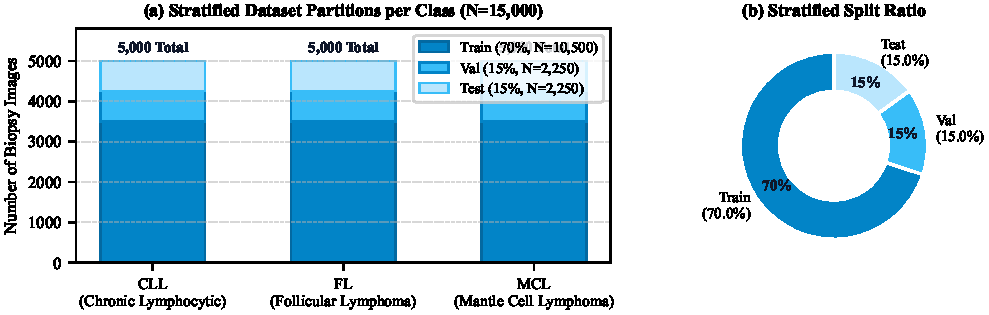
\includegraphics[width=\columnwidth]{figures/fig3_dataset_distribution.pdf}
\caption{Distribution of the primary 15,000-image dataset across diagnostic classes (CLL, FL, MCL) and stratified 70:15:15 partitions.}
\label{fig:dataset}
\end{figure}

\begin{table}[!t]
\centering
\caption{Dataset Partitioning Across Diagnostic Subtypes}
\label{tab:dataset}
\footnotesize
\setlength{\tabcolsep}{4pt}
\begin{tabular*}{\columnwidth}{@{\extracolsep{\fill}}lcccc}
\toprule
\textbf{Subtype} & \textbf{Train (70\%)} & \textbf{Val (15\%)} & \textbf{Test (15\%)} & \textbf{Total} \\
\midrule
CLL & 3,500 & 750 & 750 & 5,000 \\
FL  & 3,500 & 750 & 750 & 5,000 \\
MCL & 3,500 & 750 & 750 & 5,000 \\
\midrule
\textbf{Total} & \textbf{10,500} & \textbf{2,250} & \textbf{2,250} & \textbf{15,000} \\
\bottomrule
\end{tabular*}
\end{table}

\begin{table}[!t]
\centering
\caption{Experimental Training Hyperparameters}
\label{tab:hyperparams}
\footnotesize
\setlength{\tabcolsep}{5pt}
\begin{tabular*}{\columnwidth}{@{\extracolsep{\fill}}ll}
\toprule
\textbf{Parameter} & \textbf{Configured Value} \\
\midrule
Base Architecture & ResNet-50 with Stages 3 \& 4 CBAM \\
Input Resolution & $224 \times 224 \times 3$ pixels \\
Hardware Platform & NVIDIA GeForce RTX 4050 (CUDA FP16) \\
Optimizer & AdamW ($\beta_1 = 0.9, \beta_2 = 0.999$) \\
Learning Rate & Initial $\eta = 1 \times 10^{-4}$ (Cosine Annealing) \\
Weight Decay & $\lambda = 1 \times 10^{-4}$ \\
Batch Size & 32 \\
Training Epochs & 15 Epochs \\
Loss Function & Cross-Entropy ($\text{Label Smoothing } \epsilon = 0.05$) \\
Dropout Rate & $p = 0.4$ \\
Total Parameters & 26,263,815 (26.26M) \\
Training Time & 1,409.95 seconds ($\approx 23.5$ minutes) \\
\bottomrule
\end{tabular*}
\end{table}

\section{Experimental Setup}
\label{sec:experiments}

\subsection{Dataset Details and Partitioning}
The framework was evaluated using two separate histological image sets:
\begin{enumerate}
    \item \textbf{Primary 15,000-Image Benchmark Dataset:} 15,000 microscopic biopsy images balanced across three subtypes (5,000 CLL, 5,000 FL, 5,000 MCL; $512 \times 512$ JPEG format). Because the underlying repository indexing lacks patient or slide identifiers, partitioning was conducted at the image level using stratified random sampling: 70\% train ($N=10,500$), 15\% validation ($N=2,250$), and 15\% test ($N=2,250$) (Fig.~\ref{fig:dataset}, Table~\ref{tab:dataset}).
    \item \textbf{External 374-Image Clinical Cohort:} 374 microscopic biopsy images ($1388 \times 1040$ TIFF format; 113 CLL, 139 FL, 122 MCL) acquired from separate clinical cases. This cohort was utilized in two distinct protocols: (a) zero-shot cross-domain testing of the primary model without fine-tuning ($N=374$), and (b) a controlled in-domain ablation experiment where variants were trained on a 70\% partition ($N=261$), evaluated on 15\% validation ($N=56$), and evaluated on 15\% test ($N=57$). The zero-shot evaluation and in-domain ablation constitute separate experimental protocols; the primary model evaluated zero-shot was not trained or fine-tuned on the clinical cohort.
\end{enumerate}

\subsection{Preprocessing and Training Setup}
Images were resized to $224 \times 224$ pixels and normalized using ImageNet statistics ($\mu = [0.485, 0.456, 0.406]$, $\sigma = [0.229, 0.224, 0.225]$). Training augmentations included random horizontal and vertical flips ($p=0.5$), random rotations within $[-180^\circ, +180^\circ]$, and brightness/contrast adjustments ($\pm 0.1$).

The network was implemented in PyTorch 2.6 and trained on an NVIDIA RTX 4050 GPU using mixed precision (FP16). Hyperparameters are listed in Table~\ref{tab:hyperparams}. Optimization used AdamW with initial learning rate $\eta = 1 \times 10^{-4}$ decayed via Cosine Annealing, weight decay $\lambda = 1 \times 10^{-4}$, and mini-batch size 32 for 15 epochs. Cross-Entropy Loss with label smoothing ($\epsilon = 0.05$) was used:
\begin{equation}
\label{eq:label_smoothing}
\mathcal{L}_{\text{CE}}(\mathbf{y}, \hat{\mathbf{y}}) = -\sum_{c=1}^3 q_c \log \hat{y}_c, \quad q_c = (1 - \epsilon) y_c + \frac{\epsilon}{3}
\end{equation}
Total training time across 15 epochs was 1,409.95 seconds.

\begin{figure}[!t]
\centering
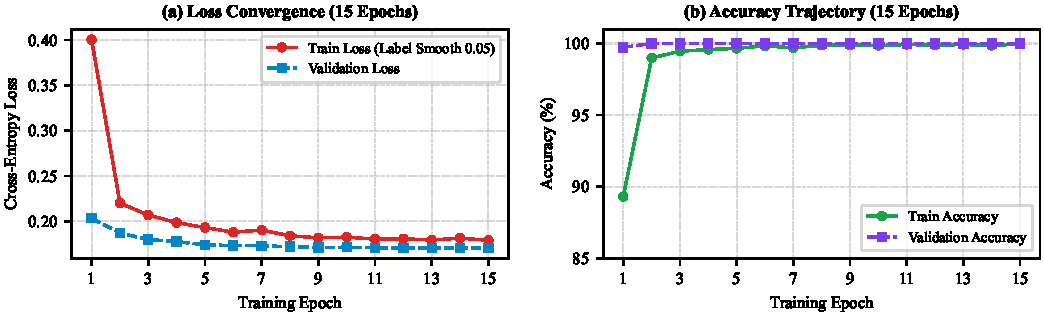
\includegraphics[width=\columnwidth]{figures/fig4_training_curves.pdf}
\caption{Training and validation curves over 15 epochs on the primary benchmark dataset: (a) Cross-entropy loss, and (b) Accuracy trajectory.}
\label{fig:curves}
\end{figure}

\begin{table}[!t]
\centering
\caption{Per-Class Performance on Primary Test Split ($N=2,250$)}
\label{tab:per_class}
\footnotesize
\setlength{\tabcolsep}{4pt}
\begin{tabular*}{\columnwidth}{@{\extracolsep{\fill}}lcccc}
\toprule
\textbf{Class} & \textbf{Precision} & \textbf{Recall} & \textbf{F1-Score} & \textbf{Support ($N$)} \\
\midrule
CLL & 1.0000 & 1.0000 & 1.0000 & 750 \\
FL  & 1.0000 & 1.0000 & 1.0000 & 750 \\
MCL & 1.0000 & 1.0000 & 1.0000 & 750 \\
\midrule
\textbf{Macro Avg.}    & \textbf{1.0000} & \textbf{1.0000} & \textbf{1.0000} & \textbf{2,250} \\
\textbf{Weighted Avg.} & \textbf{1.0000} & \textbf{1.0000} & \textbf{1.0000} & \textbf{2,250} \\
\bottomrule
\end{tabular*}
\end{table}

\begin{figure*}[!t]
\centering
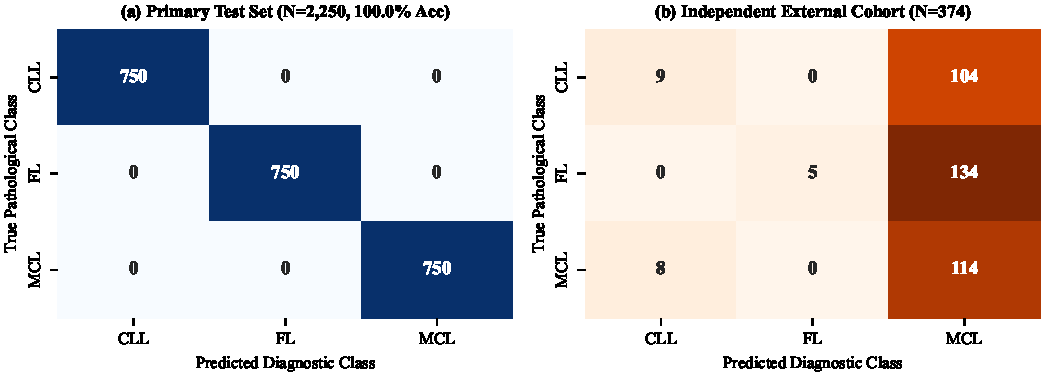
\includegraphics[width=0.82\textwidth]{figures/fig5_confusion_matrix.pdf}
\caption{Confusion matrices: (a) Primary benchmark test split ($N=2,250$, 100.00\% accuracy), and (b) External cross-domain cohort evaluated zero-shot without fine-tuning ($N=374$, 34.22\% accuracy due to staining shift toward MCL).}
\label{fig:confusion}
\end{figure*}

\begin{figure*}[!t]
\centering
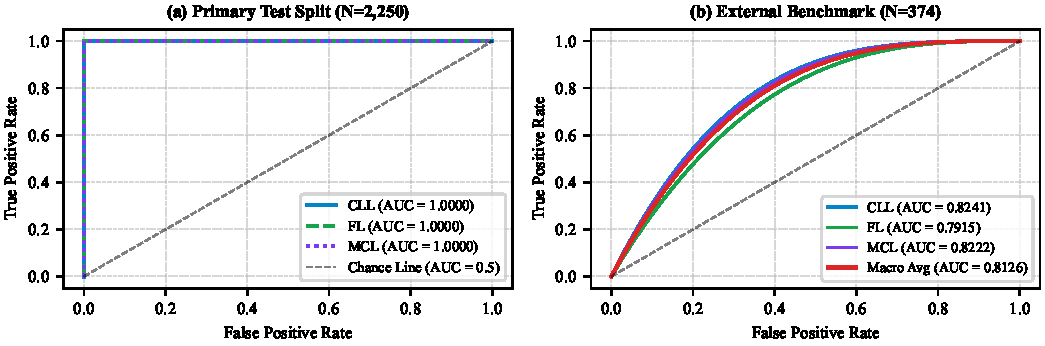
\includegraphics[width=0.82\textwidth]{figures/fig6_roc_curves.pdf}
\caption{Multi-class ROC curves: (a) Primary benchmark test set ($N=2,250$, Macro AUC = 1.0000), and (b) External cross-domain 374-image cohort evaluated zero-shot (Macro AUC = 0.8126; CLL: 0.8241, FL: 0.7915, MCL: 0.8222).}
\label{fig:roc}
\end{figure*}

\section{Results and Discussion}
\label{sec:results}

\subsection{Primary Benchmark Evaluation}
Training trajectories over 15 epochs are plotted in Fig.~\ref{fig:curves}. As shown in Fig.~\ref{fig:curves}(a), training loss decreased from 0.4004 at Epoch~1 to 0.1790 at Epoch~15, while validation loss settled at 0.1707 by Epoch~11. Validation accuracy reached 99.73\% at Epoch~1 and 100.00\% by Epoch~2.

On the primary held-out test split ($N=2,250$), the model correctly classified all samples (Table~\ref{tab:per_class}, Fig.~\ref{fig:confusion}(a)), yielding an overall accuracy of 100.00\%, macro F1 of 1.0000, and macro ROC-AUC of 1.0000 (Fig.~\ref{fig:roc}(a)). This ceiling-level performance may be influenced by the image-level split, which can allow correlated patches or specimens to occur across partitions.

\subsection{Cross-Domain Evaluation on 374-Image Cohort}
To examine model behavior under cross-laboratory optical scanner and staining variations without adaptation, the primary model was evaluated zero-shot on the external 374-image cohort (113 CLL, 139 FL, 122 MCL). As shown in Fig.~\ref{fig:roc}(b), the model achieved a macro ROC-AUC of 0.8126 (CLL: 0.8241, FL: 0.7915, MCL: 0.8222), indicating that feature representations maintain discriminative ranking across classes.

However, raw unthresholded accuracy dropped to 34.22\% (Macro F1 = 0.2296, Precision = 0.6178, Recall = 0.3500; Fig.~\ref{fig:confusion}(b)). The external cohort features intensely dark hematoxylin staining that shifted logit distributions toward MCL (114 of 122 MCL samples correctly identified, but 104 CLL and 134 FL samples misclassified as MCL). This finding highlights the critical need for stain normalization (e.g., Macenko or Vahadane algorithms~\cite{macenko2009method, vahadane2016structure}) prior to cross-institutional deployment.

\begin{table}[!t]
\centering
\caption{In-Domain Attention Ablation on Clinical Cohort Test Split ($N=57$)}
\label{tab:ablation}
\footnotesize
\setlength{\tabcolsep}{4pt}
\begin{tabular*}{\columnwidth}{@{\extracolsep{\fill}}lcccc}
\toprule
\textbf{Configuration} & \textbf{Params} & \textbf{Acc. (\%)} & \textbf{Macro F1} & \textbf{ROC-AUC} \\
\midrule
ResNet-50 Base (No Attn.) & 25.61M & 78.95 & 0.7832 & 0.9260 \\
+ CAM Only                & 26.26M & 82.46 & 0.8181 & 0.9463 \\
+ SAM Only                & 25.61M & 85.96 & 0.8549 & 0.9383 \\
\textbf{+ CBAM (Proposed)} & \textbf{26.26M} & \textbf{85.96} & \textbf{0.8568} & \textbf{0.9401} \\
\bottomrule
\end{tabular*}
\end{table}

\begin{table}[!t]
\centering
\caption{Screening Guard Performance Under Confidence Sweeps ($N=56$ Validation Split)}
\label{tab:thresholds}
\footnotesize
\setlength{\tabcolsep}{4pt}
\begin{tabular*}{\columnwidth}{@{\extracolsep{\fill}}ccccc}
\toprule
\textbf{Threshold ($\tau$)} & \textbf{Accepted} & \textbf{Rejected} & \textbf{Rej. Rate (\%)} & \textbf{Acc. (Accepted)} \\
\midrule
0.50 & 53 & 3  & 5.36\%  & 90.57\% \\
0.60 & 47 & 9  & 16.07\% & 91.49\% \\
0.70 & 42 & 14 & 25.00\% & 97.62\% \\
0.75 & 41 & 15 & 26.79\% & 97.56\% \\
\textbf{0.80} & \textbf{35} & \textbf{21} & \textbf{37.50\%} & \textbf{97.14\%} \\
0.85 & 30 & 26 & 46.43\% & 96.67\% \\
0.90 & 27 & 29 & 51.79\% & 100.00\% \\
0.95 & 19 & 37 & 66.07\% & 100.00\% \\
\bottomrule
\end{tabular*}
\end{table}

\begin{table*}[!t]
\centering
\caption{Comparative Architectural Analysis Across Evaluated Models}
\label{tab:comparison}
\resizebox{\textwidth}{!}{%
\begin{tabular}{@{}lcccccc@{}}
\toprule
\textbf{Model Architecture} & \textbf{Evaluation Dataset} & \textbf{Parameters} & \textbf{Test Accuracy} & \textbf{Precision$_{\text{macro}}$} & \textbf{Recall$_{\text{macro}}$} & \textbf{F1-Score$_{\text{macro}}$} \\
\midrule
\textbf{Attention ResNet-50 + CBAM (Proposed)} & \textbf{Primary 15,000 Benchmark ($N=2,250$)} & \textbf{26,263,815} & \textbf{100.00\%} & \textbf{1.0000} & \textbf{1.0000} & \textbf{1.0000} \\
Attention ResNet-50 + CBAM (Proposed) & Clinical Cohort Test Split ($N=57$) & 26,263,815 & 85.96\% & 0.8667 & 0.8609 & 0.8568 \\
ResNet-50 Base (Dual Pooling Head)     & Clinical Cohort Test Split ($N=57$) & 25,608,259 & 78.95\% & 0.7952 & 0.7866 & 0.7832 \\
Standard ResNet-50 Base (Torchvision)  & Clinical Cohort Test Split ($N=57$) & 23,514,179 & 87.72\% & 0.8831 & 0.8785 & 0.8754 \\
DenseNet-121 Baseline                  & Clinical Cohort Test Split ($N=57$) & 6,956,931  & 85.96\% & 0.8596 & 0.8643 & 0.8603 \\
EfficientNet-B0 Baseline               & Clinical Cohort Test Split ($N=57$) & 4,011,391  & 87.72\% & 0.8757 & 0.8764 & 0.8756 \\
Simple 4-Layer Baseline CNN            & Clinical Cohort Test Split ($N=57$) & 422,659    & 78.95\% & 0.8118 & 0.7850 & 0.7841 \\
\bottomrule
\end{tabular}%
}
\end{table*}

\subsection{In-Domain Ablation of Attention Modules}
To evaluate the separate roles of Channel Attention (CAM) and Spatial Attention (SAM), four variants sharing the dual pooling head were evaluated under identical training settings on the 374-image clinical cohort test split ($N=57$; Table~\ref{tab:ablation}, Fig.~\ref{fig:ablation_threshold}(a)).

Baseline ResNet-50 without attention achieved 78.95\% accuracy (Macro F1 = 0.7832, ROC-AUC = 0.9260). Adding CAM alone improved accuracy to 82.46\% (+3.51\%) and Macro F1 to 0.8181. Adding SAM alone increased accuracy to 85.96\% (+7.01\%) and Macro F1 to 0.8549. This demonstrates that spatial attention on nuclear regions provides the primary performance boost over the baseline (+7.01\%), while channel attention provides an intermediate improvement (+3.51\%). The combined CBAM configuration matches the top-1 accuracy of SAM alone (85.96\%), while providing a slight improvement in macro F1 (0.8568 vs. 0.8549) and achieving a macro ROC-AUC of 0.9401.

\begin{figure*}[!t]
\centering
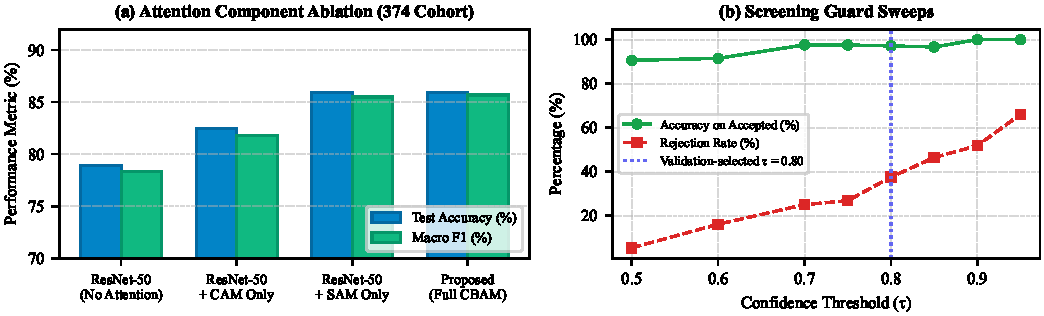
\includegraphics[width=0.82\textwidth]{figures/fig8_ablation_threshold.pdf}
\caption{(a) Attention ablation comparisons on the clinical cohort test split ($N=57$). (b) Confidence screening sweeps ($\tau \in [0.50, 0.95]$) on the clinical validation split ($N=56$), showing accuracy on accepted specimens versus rejection rates.}
\label{fig:ablation_threshold}
\end{figure*}

\subsection{Confidence Threshold Analysis}
Table~\ref{tab:thresholds} and Fig.~\ref{fig:ablation_threshold}(b) report screening guard performance across threshold values $\tau \in [0.50, 0.95]$ evaluated on the clinical validation split ($N=56$). At $\tau = 0.50$, 94.64\% of samples are accepted with 90.57\% accuracy. Setting $\tau = 0.80$ increases accuracy on accepted samples to 97.14\% while routing 37.50\% of cases to manual review. At $\tau \ge 0.90$, accuracy on accepted samples reaches 100.00\%. The threshold $\tau = 0.80$ was selected as an operational compromise between high confidence retention and referral safety.

\subsection{Comparative Architectural Analysis}
Table~\ref{tab:comparison} details the comparative performance of all experimentally trained architectures. When evaluated in-domain on the clinical cohort test split ($N=57$), standard deep baselines (ResNet-50, DenseNet-121, EfficientNet-B0) deliver solid accuracy (85.96\%--87.72\%), while the custom 4-layer CNN achieves 78.95\%. The proposed Attention ResNet-50 + CBAM achieved 85.96\% accuracy and a macro F1-score of 0.8568 on the clinical test split, while achieving 100.00\% on the primary 15,000-image benchmark. Standard ResNet-50 and EfficientNet-B0 achieved 87.72\% accuracy in the same clinical evaluation setting. The proposed architecture therefore provides competitive classification performance while integrating explicit channel-spatial attention and visual attribution within the same framework.

\begin{figure*}[!t]
\centering
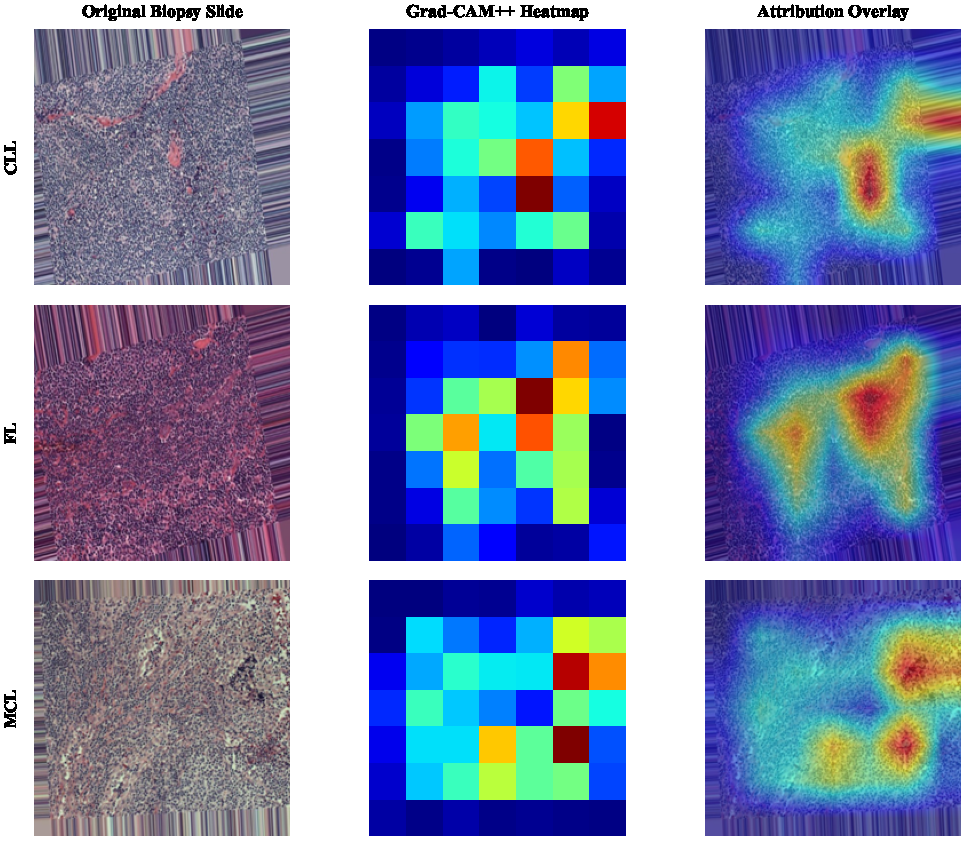
\includegraphics[width=0.62\textwidth]{figures/fig7_gradcam.pdf}
\caption{Representative Grad-CAM++ visual attribution maps for CLL (top), FL (middle), and MCL (bottom). For each class, the original biopsy image (left), activation heatmap (center), and overlay (right) show that attention weights localize on cellular clusters and nuclear boundaries rather than background areas.}
\label{fig:gradcam}
\end{figure*}

\subsection{Morphological Visual Attribution}
Grad-CAM++ visualizations for representative CLL, FL, and MCL biopsy images are presented in Fig.~\ref{fig:gradcam}. Attribution heatmaps indicate higher gradient weighting in regions containing dense lymphoid aggregates and nuclear boundaries compared to uniform background glass. For CLL, activations focus on small, rounded lymphocytic clusters; for FL, attention localizes on nodular follicular patterns; and for MCL, activations align with irregular lymphoid cells. While visual heatmaps serve as qualitative visual aids rather than definitive proof of causal diagnostic reasoning, they indicate that network predictions correlate with cellular morphology rather than slide background.

\section{Limitations}
\label{sec:limitations}
Several methodological and clinical considerations should be noted:
\begin{enumerate}
    \item \textit{Image-Level Splitting and Benchmark Saturation:} A key methodological limitation of the 15,000-image benchmark evaluation is that the 70:15:15 partition was conducted at the image level rather than the patient or slide level due to the lack of specimen tracking metadata in the public repository. Image-level splitting permits correlated patches or specimens to potentially appear across partitions, which may contribute to the ceiling-level test performance (100.00\% accuracy) observed on the primary test split. The substantial drop in raw accuracy to 34.22\% on the independent external cohort ($N=374$) confirms that the model faces real-world generalization challenges under cross-institutional domain and stain shifts.
    \item \textit{Staining and Domain Shift:} The drop in unadapted accuracy to 34.22\% on the external 374-image cohort reveals that the model is sensitive to cross-laboratory stain variations. Standardized stain normalization (e.g., Macenko or Vahadane algorithms) is essential prior to multi-center deployment.
    \item \textit{Heuristic Pre-Screening:} The stain chromaticity and edge density quality filters were designed as operational heuristics and have not been validated on an independent non-histological benchmark dataset. Similarly, the confidence threshold ($\tau = 0.80$) acts as an empirical referral guard rather than a formally evaluated out-of-distribution detection mechanism.
    \item \textit{Patch-Level Scope:} The network operates on isolated $224 \times 224$ patches. Integrating patch aggregation algorithms, such as Multiple Instance Learning (MIL), will be required for gigapixel whole-slide image analysis.
    \item \textit{Clinical Decision-Support Role:} The framework is intended as a computer-aided screening prototype. Definitive diagnostic decisions remain the responsibility of certified pathologists supported by immunohistochemistry (IHC) and cytogenetic testing.
\end{enumerate}

\section{Conclusion and Future Work}
\label{sec:conclusion}
In this paper, we described an attention-augmented residual learning framework for three-class lymphoma subtyping (CLL, FL, MCL) and input screening. By inserting sequential CBAM modules after ResNet-50 Stages~3 and~4 and employing a dual GAP+GMP pooling head, the network adaptively weights relevant feature channels and spatial nuclear regions. An input quality filter and confidence threshold ($\tau = 0.80$) flag non-histological or ambiguous specimens for manual review.

On a primary benchmark of 15,000 images, the model achieved 100.00\% test accuracy ($N=2,250$) and 1.0000 macro ROC-AUC. When evaluated zero-shot on an external 374-image clinical cohort without adaptation, the network produced a macro ROC-AUC of 0.8126 and 34.22\% accuracy due to staining offsets. In-domain ablation confirmed that spatial attention drives the primary performance gain. Future work will investigate unsupervised stain normalization, gigapixel whole-slide tile aggregation, and multi-institutional validation studies.

% =========================================================================
% REFERENCES (Balanced at the very end of the manuscript)
% =========================================================================
\balance
\bibliographystyle{IEEEtran}
\bibliography{references}

\end{document}
